%=============================================================================
\documentclass[10pt,a4paper]{article}
%
%
%
\usepackage{graphicx}
\usepackage{hyperref}
\usepackage{verbatim}
\usepackage{fix-cm}
\usepackage{lineno}
\usepackage{fancyhdr}
%
\usepackage{amsmath}
%
\oddsidemargin  0.1 in
\evensidemargin 0.1 in
%
%
\newlength{\backindent}\setlength{\backindent}{2cm}
\textwidth 5.375 in % Width of text line.
\advance\textheight by1.4cm
\advance\voffset by-1.4cm
\advance\textwidth by\backindent
%
%
% === Fancy headers setup  ===============================
%
\setlength{\headheight}{15.2pt}
\pagestyle{fancyplain} {
\fancyhead[L]{
\includegraphics[height=10mm]{DD4hep-AIDA-logo.png}\vspace{-0.3cm}}
\fancyhead[C]{}
\fancyhead[R]{\sffamily{\underline{\hspace{6cm}Advanced European Infrastructures for Detectors at Accelerators}}}
\fancyfoot[L]{}
\fancyfoot[C]{\sffamily{User Manual}}
\fancyfoot[R]{\sffamily{\thepage}}
}
%
%
\newcommand{\tw}[1]{${\tt{#1}}$}
\newcommand{\tts}[1]{{\tt\small{#1}}}
\newcommand{\bold}[1]{{\bf{#1}}}
%
%
\newcommand{\DDE}{{$\tt{DDEve}$\space}}
\newcommand{\DDhep}{{$\tt{DD4hep}$\space}}
\newcommand{\DDH}{{$\tt{DD4hep}$\space}}
\newcommand{\DDG}{{\tt{DDG4}\space}}
\newcommand{\DDA}{{\tt{DDAlign}\space}}
\newcommand{\DDR}{{\tt{DDRec}\space}}
%
%
\newcommand{\docline}[2]{\vspace{0.1cm}{\bf{#1}} & \parbox{14.5cm}{#2}\\}
%
% === Specialization of the lineno package
%
\renewcommand{\linenumberfont} {\normalfont\small\sffamily}
\renewcommand{\makeLineNumber} {\makeLineNumberLeft}
\renewcommand{\linenumbersep} {2pt}
%
% === Set font to code section with line numbers
%
\newenvironment{code}{\par\vspace{0.01cm}\small\linenumbers\verbatim\setcounter{linenumber}{1}}{\endverbatim\nolinenumbers\vspace{-0.02cm}}%
%
% === Set font to code section with line numbers
%
\newenvironment{unnumberedcode}{\par\vspace{-0.1cm}\small\verbatim\setcounter{linenumber}{1}}%
{\endverbatim\vspace{-0.2cm}}
%
% === Command to insert http links to the DD4hep geomtery package
%
\newcommand{\detdesc}[2]
{
    \href{http://www.cern.ch/frankm/DD4hep/#1}{#2}
}
%
% === Command to insert http links to the ROOT geomtery package
%
\newcommand{\tgeo}[2]
{
    \href{http://root.cern.ch/root/html/#1.html}{#2}
}
\newcommand{\tgeoO}[3]
{
    \href{http://root.cern.ch/root/html/#1:#2}{#3}
}
%
% ===  Compactify the item list  =========================
%
\newcommand{\itemcompact}{\setlength{\itemsep}{1pt}\setlength{\parskip}{0pt}\setlength{\parsep}{0pt}}
%
%
% ===  Title page command  ===============================
%
%
\newcommand{\basictitle}[2]{
%
\pagestyle{empty}
%

\includegraphics[height=25mm] {DD4hep-AIDA-logo.png}

\vspace{0.02cm}

{\sffamily{\underline{\hspace{6cm}Advanced European Infrastructures for Detectors at Accelerators}}}

\vspace{2cm}

\begin{center}
{\fontsize{72}{32}\selectfont{\bfseries{#1}}}

\vspace{3cm}
{\Huge\bf{#2}}
\vspace{3cm}

\end{center}
}


\newcommand{\mytitle}[3]{
\begin{titlepage}
\basictitle{#1}{#2}
\begin{center}
{#3}

%%M.Frank %%\textsuperscript{1}
%%%F.Gaede\textsuperscript{2},
%%%C.Grefe\textsuperscript{1}
%%\vspace{1cm}
%%\textsuperscript{1}
%%{CERN, 1211 Geneva 23, Switzerland}
%%%{\textsuperscript{2} {Desy, 22607 Hamburg, Germany}
\end{center}
\end{titlepage}
}

%
\pagestyle{fancyplain}{\fancyfoot[C]{\sffamily{DDAlign User Manual}}}
%
\begin{document}   
%
\mytitle{
DDCond
}{
Conditions Support for the \\
\vspace{0.5cm}
DD4hep Geometry Description \\
\vspace{0.5cm}
Toolkit
\vspace{2cm}
}{DDAlign User Manual}
%
%
%==  Abstract  ===============================================================
\pagestyle{plain}
\pagenumbering{Roman}
\setcounter{page}{1}
\begin{abstract}
%=============================================================================

\noindent
\normalsize
Experimental setups in High Energy Physics are highly complex assemblies 
consisting of various detector devices typically called {\it{subdetectors}}.
Contrary to the ideal world, where all these components are of perfect shape 
and at exact positions, existing devices have imperfections both in their 
shape and their relative and absolute positions.\\
To still measure the detector response from particle collisions with the highest
possible precision, these imperfections are taken into account when converting
measured signals to space-points in the measurement devices. This procedure
is called {\it{detector alignment}}. \DDhep does not want to solve the exact 
problem of the detector alignment itself, but rather support firstly algorithms 
determining the imperfections and secondly support the application of the 
measured imperfection to the ideal geometry for further event data processing.\\
We will present the tools to support the detector alignment procedures using 
the \DDhep detector description toolkit. 
The \DDA toolkit implements a modular and flexible approach to introduce and
access the imperfections.\\
The design is strongly driven by easy of use;
developers of detector descriptions and applications using
them should provide minimal information and minimal specific
code to achieve the desired result.

\end{abstract}

\vspace{8cm}

\begin{center}
{\large{\bf{
\begin{tabular} {| l | l | l |}
\hline
\multicolumn{3}{| c |}{} \\[0.2cm]
\multicolumn{3}{| c |}{Document History} \\[0.2cm]
\multicolumn{3}{| c |}{} \\[0.2cm]
\hline
                 &      &        \\
Document         &      &        \\
version          & Date & Author \\[0.2cm] \hline
                 &      &        \\
1.0              & 10/4/2014 & Markus Frank CERN/LHCb  \\
                 &      &        \\        \hline 
\end{tabular}
}}}
\end{center}

\clearpage
%
%
%==  TOC  ====================================================================
\tableofcontents
\clearpage
%
%
%=============================================================================
% Manual
%=============================================================================
\pagenumbering{arabic}
\setcounter{page}{1}

%=============================================================================
\section{Introduction}
\label{sec:ddalign-user-manual-introduction}
%=============================================================================
\noindent
This manual should introduce to the \DDA framework. 
One goal of \DDA is to easily model geometrical imperfections applied to
the ideal geometry of detection devices as they are typically used in 
high energy physics experiments.

\noindent
\DDA formalizes both the access and the application of geometrical imperfection 
to the ideal geometry. In this manual we will shortly describe the model used
to describe an experiments detector description and then in more detail 
document the support for alignment with its programming interfaces.

%=============================================================================
\begin{figure}[h]
  \begin{center}
    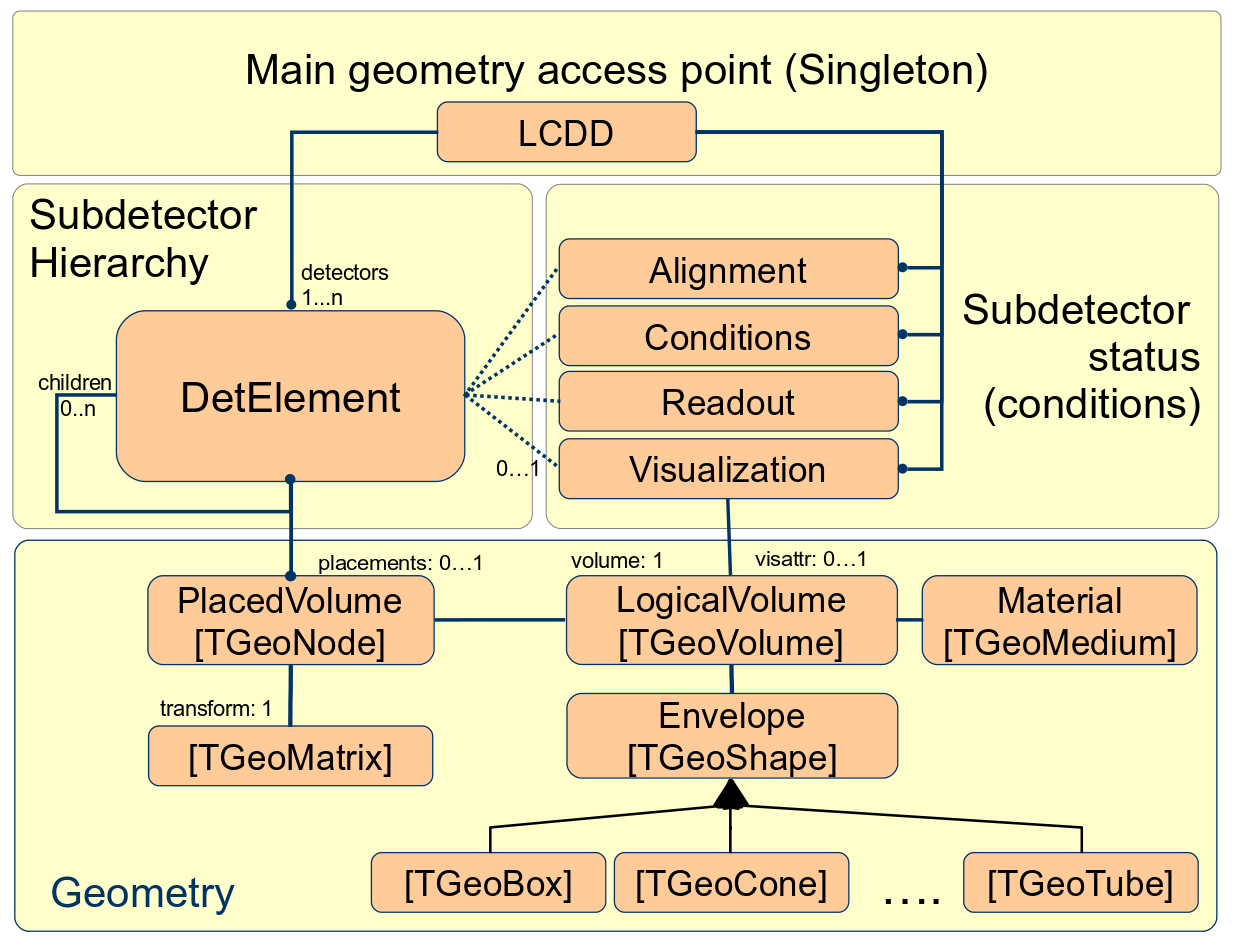
\includegraphics[height=90mm] {DD4hep_classes.png}
    \caption{Class diagram with the main classes and their relations 
             for the Generic Detector Description Model. The implementing
             ROOT classes are shown in brackets.}
    \label{fig:dd4hep-detector-model}
  \end{center}
\end{figure}
\vspace{-0.5cm}
%=============================================================================
\subsection{Generic Detector Description Model}
\label{subsec:generic-model}
%=============================================================================

\noindent
This is the heart of the DD4hep detector description toolkit. Its purpose is 

\newpage
%=============================================================================
\begin{thebibliography}{9}
\bibitem{bib:LHCb-geometry} S. Ponce et al., 
                "Detector Description Framework in LHCb", 
                International Conference on Computing in High Energy and Nuclear Physics  (CHEP 2003), 
                La Jolla, CA, 2003, proceedings. 
\end{thebibliography}
%=============================================================================
\end{document}
